\section{Testing}
\subsection{Analisi statica}
Per l'analisi statica del codice Java è stato utilizzato il tool STAN4J, integrato nel IDE Eclipse. Il report è riportato a fine capitolo.

\subsection{Analisi dinamica}
Nell'iterazione 4 si sono testate tutte le API Rest implementate, utlizzando Postman (\Fig \ref{}). In particolare si sono testate le seguenti funzionalità:


\clearpage

\subsection{Unit Test}
\subsubsection{LvsEmergency Server}



\clearpage

\subsubsection{Client App}
Lato client è stata testata la corretta creazione della classe \texttt{Position} a partire da una stringa JSON. Di seguito è riportato il codice del test: 

\lstinputlisting[language=C++]{./Iterazione 4/OtherFiles/testcpp.cpp}

Il risultato dei test ha confermato il corretto funzionamento delle nuove funzioni e di quelle precedenti. 

\begin{figure}[h!]
	\centering
	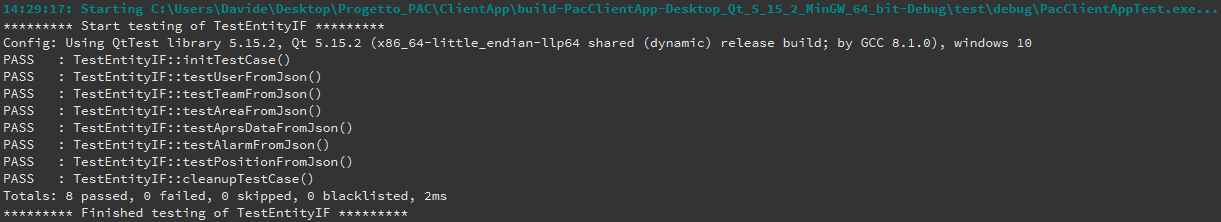
\includegraphics[width=1\linewidth]{./Iterazione 4/ImageFiles/testcpp}
	\caption{Risultato test con Qt Test.}
	\label{fig:RisultatiTestQtIT4}
\end{figure}
\clearpage

\section{Documentazione API}
